\section{Divide et Impera}

\subsection{Definizione}
Il paradigma \textbf{divide et impera} risolve un problema tramite tre passi:
\begin{enumerate}
	\item \textbf{Divide}: suddividere l'istanza in sottoistanze più piccole.
	\item \textbf{Impera}: risolvere ricorsivamente le sottoistanze.
	\item \textbf{Combina}: comporre le soluzioni parziali nella soluzione finale.
\end{enumerate}

Schema generale (coerente con le slide): \newline
\begin{algorithm}[H]
	\caption{DivideEtImpera$(X)$}
	\KwIn{$X$ istanza di dimensione $|X|=n$}
	\KwOut{$Y$ soluzione}
	\If{$|X|\le n_0$}{
		\Return \texttt{adhoc}$(X)$\;
	}
	Dividi $X$ in sottoistanze $X_1,\dots,X_a$\;
	\For{$i\gets1$ \KwTo $a$}{
		$Y_i\gets$ DivideEtImpera$(X_i)$\;
	}
	Combina $Y_1,\dots,Y_a$ in $Y$\;
	\Return $Y$\;
\end{algorithm}

\subsection{Intuizione}
La tecnica è efficace quando i sottoproblemi sono il più possibile disgiunti e il costo di combinazione non domina il costo ricorsivo.

\subsection{Motivazione}
Molti problemi importanti (prodotto di interi grandi, MergeSort, massimo sottoarray) ammettono una decomposizione naturale che rende il costo asintotico inferiore rispetto ad approcci diretti.

\subsection{Algoritmo}
Il costo si modella tramite una ricorrenza:
\[
T(n)=
\begin{cases}
\;g(n) & n\le n_0,\\
\;a\,T(n/b)+f(n) & \text{altrimenti},
\end{cases}
\]
dove:
\begin{itemize}
	\item $g(n)$ è il costo del caso base (\texttt{adhoc}),
	\item $f(n)$ è il costo non ricorsivo (divide + combina),
	\item $a$ è il numero di sottoistanze,
	\item $n/b$ è la dimensione tipica di ciascuna sottoistanza.
\end{itemize}

\subsection{Esempio guidato}
\paragraph{Prodotto di interi (Karatsuba/Gauss).}
Siano $x=2^{n/2}x_L+x_R$ e $y=2^{n/2}y_L+y_R$.
Formula base:
\[
xy=2^n(x_Ly_L)+2^{n/2}(x_Ly_R+x_Ry_L)+x_Ry_R.
\]
Con il trucco di Gauss:
\[
P_1=x_Ly_L,\quad P_2=x_Ry_R,\quad P_3=(x_L+x_R)(y_L+y_R),
\]
\[
xy=2^nP_1+2^{n/2}(P_3-P_1-P_2)+P_2.
\]
Quindi le moltiplicazioni ricorsive diventano 3 (non 4):
\[
T(n)=3T(n/2)+\Theta(n)=\Theta(n^{\log_2 3}).
\]

\begin{algorithm}[H]
	\caption{\textsc{Prodotto}$(x,y)$}
	\KwIn{$x,y$ interi non negativi di $n=2^l$ bit}
	\KwOut{Prodotto $xy$}
	\If{$n\le 64$}{
		\Return $xy$\tcp*{caso base $\Theta(1)$}
	}
	$x_L\gets$ $n/2$ bit più significativi di $x$;\;
	$x_R\gets$ $n/2$ bit meno significativi di $x$\;
	$y_L\gets$ $n/2$ bit più significativi di $y$;\;
	$y_R\gets$ $n/2$ bit meno significativi di $y$\tcp*{Divide, $\Theta(n)$}
	$P_1\gets\textsc{Prodotto}(x_L,y_L)$\;
	$P_2\gets\textsc{Prodotto}(x_R,y_R)$\;
	$P_3\gets\textsc{Prodotto}(x_L+x_R,y_L+y_R)$\tcp*{Impera, $3T(n/2)$}
	\Return $(P_1\ll n)+((P_3-P_1-P_2)\ll n/2)+P_2$\tcp*{Combina, $\Theta(n)$}
\end{algorithm}

\paragraph{MergeSort.}
\[
T(n)=2T(n/2)+\Theta(n)=\Theta(n\log n).
\]

\paragraph{Massimo sottoarray (versione divide et impera).}
La soluzione su $A[low:high]$ è il massimo tra:
\begin{enumerate}
	\item massimo interamente a sinistra,
	\item massimo interamente a destra,
	\item massimo che attraversa $mid$.
\end{enumerate}
Ricorrenza:
\[
T(n)=2T(n/2)+\Theta(n)=\Theta(n\log n).
\]

\begin{definizione}[Massimo sottoarray]
	Dato $A[1:n]$, il \textbf{massimo sottoarray} è un sottoarray non vuoto
	$A[i:j]$ ($1\le i\le j\le n$) la cui somma
	\[
	\sum_{t=i}^{j} A[t]
	\]
	è massima.
\end{definizione}

\begin{esempio}[Profitti annuali (slide)]
	Profitti di una società negli anni 2001--2012:
	\[
	A=\langle 3,10,15,1,-25,32,-5,10,1,2,3,-2\rangle.
	\]
	Dal 2001 al 2003: $3+10+15=33$; dal 2006 al 2010: $1-25+32-5+10=13$;
	dal 2008 al 2010: $32-5+10=37$, che è anche il massimo globale.
\end{esempio}

\begin{algorithm}[H]
	\caption{\textsc{MassimoSottoarrayForzaBruta}$(A)$}
	\KwIn{Array $A[1:n]$}
	\KwOut{Coppia $(i,j)$ e somma massima}
	$\mathit{somma}\gets-\infty$\;
	\For{$i\gets 1$ \KwTo $n$}{
		\For{$j\gets i$ \KwTo $n$}{
			$s\gets 0$\;
			\For{$t\gets i$ \KwTo $j$}{$s\gets s+A[t]$}
			\If{$s>\mathit{somma}$}{
				$\mathit{somma}\gets s$;\;
				$\mathit{best}\gets(i,j)$\;
			}
		}
	}
	\Return $(\mathit{best},\mathit{somma})$\;
\end{algorithm}
Complessità: $\binom{n+1}{2}=\Theta(n^2)$ coppie $(i,j)$ e somma in $O(n)$ per coppia $\Rightarrow\Theta(n^3)$ nel caso peggiore (anche $\Omega(n^2)$).

\begin{algorithm}[H]
	\caption{\textsc{Find-Max-Crossing-Subarray}$(A,\mathit{low},\mathit{mid},\mathit{high})$}
	\KwIn{Array $A$, indici $\mathit{low},\mathit{mid},\mathit{high}$}
	\KwOut{Indici del massimo sottoarray che attraversa $\mathit{mid}$ e relativa somma}
	$\mathit{left\_sum}\gets-\infty$;\; $s\gets 0$\;
	$i\gets \mathit{mid}$\;
	\While{$i\ge \mathit{low}$}{
		$s\gets s+A[i]$\;
		\If{$s>\mathit{left\_sum}$}{$\mathit{left\_sum}\gets s$;\; $\mathit{max\_left}\gets i$}
		$i\gets i-1$\;
	}
	$\mathit{right\_sum}\gets-\infty$;\; $s\gets 0$\;
	\For{$j\gets \mathit{mid}+1$ \KwTo $\mathit{high}$}{
		$s\gets s+A[j]$\;
		\If{$s>\mathit{right\_sum}$}{$\mathit{right\_sum}\gets s$;\; $\mathit{max\_right}\gets j$}
	}
	\Return $(\mathit{max\_left},\mathit{max\_right},\mathit{left\_sum}+\mathit{right\_sum})$\;
\end{algorithm}

\begin{algorithm}[H]
	\caption{\textsc{Find-Maximum-Subarray}$(A,\mathit{low},\mathit{high})$}
	\KwIn{Array $A$, estremi $\mathit{low},\mathit{high}$}
	\KwOut{Massimo sottoarray in $A[\mathit{low}:\mathit{high}]$}
	\If{$\mathit{low}=\mathit{high}$}{
		\Return $(\mathit{low},\mathit{high},A[\mathit{low}])$\;
	}
	$\mathit{mid}\gets\lfloor(\mathit{low}+\mathit{high})/2\rfloor$\;
	$(l_1,h_1,s_1)\gets\textsc{Find-Maximum-Subarray}(A,\mathit{low},\mathit{mid})$\;
	$(l_2,h_2,s_2)\gets\textsc{Find-Maximum-Subarray}(A,\mathit{mid}+1,\mathit{high})$\;
	$(l_c,h_c,s_c)\gets\textsc{Find-Max-Crossing-Subarray}(A,\mathit{low},\mathit{mid},\mathit{high})$\;
	\Return il terzetto con somma massima tra $(l_1,h_1,s_1)$, $(l_2,h_2,s_2)$, $(l_c,h_c,s_c)$\;
\end{algorithm}
La chiamata iniziale è \textsc{Find-Maximum-Subarray}$(A,1,n)$.

\subsection{Grafico o diagramma}
\begin{center}
\begin{verbatim}
                 T(n)
              /        \
         T(n/2)       T(n/2)
         /   \         /   \
     T(n/4) T(n/4)  T(n/4) T(n/4)
\end{verbatim}
\end{center}

Esempio di albero di ricorsione per
\[
T(n)=3T(\lfloor n/4\rfloor)+\Theta(n^2):
\]
\begin{center}
\begin{verbatim}
Livello i:
- numero nodi: 3^i
- costo per nodo: c (n/4^i)^2
- costo livello: (3/16)^i c n^2
\end{verbatim}
\end{center}

\begin{figure}[H]
	\centering
	\begin{tikzpicture}[
		level distance=11mm,
		level 1/.style={sibling distance=42mm},
		level 2/.style={sibling distance=21mm},
		every node/.style={draw, primary, rounded corners, font=\small,
			minimum width=1.1cm, inner sep=2pt}
		]
		\node {$T(n)$}
		child { node {$T(n/2)$}
			child { node {$T(n/4)$} }
			child { node {$T(n/4)$} }
		}
		child { node {$T(n/2)$}
			child { node {$T(n/4)$} }
			child { node {$T(n/4)$} }
		};
	\end{tikzpicture}
	\caption{Albero di ricorsione tipico per $T(n)=2T(n/2)+\Theta(n)$ (es.\ MergeSort, massimo sottoarray).}
\end{figure}

\begin{figure}[H]
	\centering
	\begin{tikzpicture}[
		level distance=11mm,
		level 1/.style={sibling distance=50mm},
		level 2/.style={sibling distance=16mm},
		every node/.style={draw, primary, rounded corners, font=\small,
			minimum width=1.0cm, inner sep=2pt}
		]
		\node {$T(n)$}
		child { node {$T(n/2)$}
			child { node {$T(n/4)$} }
			child { node {$T(n/4)$} }
			child { node {$T(n/4)$} }
		}
		child { node {$T(n/2)$}
			child { node {$T(n/4)$} }
			child { node {$T(n/4)$} }
			child { node {$T(n/4)$} }
		};
	\end{tikzpicture}
	\caption{Albero di ricorsione per \textsc{Prodotto} (Karatsuba): $T(n)=3T(n/2)+\Theta(n)$.}
\end{figure}

\begin{figure}[H]
	\centering
	\begin{tikzpicture}[
		level distance=9mm,
		level 1/.style={sibling distance=38mm},
		level 2/.style={sibling distance=12mm},
		every node/.style={draw, primary, font=\footnotesize,
			minimum width=0.9cm, inner sep=1pt}
		]
		\node[align=center] {$T(n)$\\$\Theta(n^2)$}
		child { node {$T(\lfloor n/4\rfloor)$}
			child { node {$\cdots$} }
			child { node {$\cdots$} }
			child { node {$\cdots$} }
		}
		child { node {$T(\lfloor n/4\rfloor)$}
			child { node {$\cdots$} }
			child { node {$\cdots$} }
			child { node {$\cdots$} }
		}
		child { node {$T(\lfloor n/4\rfloor)$}
			child { node {$\cdots$} }
			child { node {$\cdots$} }
			child { node {$\cdots$} }
		};
		\node[font=\scriptsize, below=6mm of current bounding box.south]
		{livello $i$: $3^i$ nodi, costo per nodo $\Theta\!\bigl((n/4^i)^2\bigr)$,
			costo livello $\bigl(\frac{3}{16}\bigr)^i\Theta(n^2)$};
	\end{tikzpicture}
	\caption{Albero di ricorsione per $T(n)=3T(\lfloor n/4\rfloor)+\Theta(n^2)$: somma geometrica $\Rightarrow O(n^2)$.}
\end{figure}

\subsection{Dimostrazione}
\begin{teorema}[Teorema dell'esperto]
	Date costanti $a>0$, $b>1$ e una funzione $f(n)$ \emph{forzante} (asintoticamente positiva), per
	\[
	T(n)=aT(n/b)+f(n)
	\]
	vale:
	\begin{enumerate}
	\item Se $f(n)=O\!\left(n^{\log_b a-\varepsilon}\right)$, allora
	\[
	T(n)=\Theta\!\left(n^{\log_b a}\right).
	\]
	\item Se $f(n)=\Theta\!\left(n^{\log_b a}\log^k n\right)$, allora
	\[
	T(n)=\Theta\!\left(n^{\log_b a}\log^{k+1}n\right).
	\]
	\item Se $f(n)=\Omega\!\left(n^{\log_b a+\varepsilon}\right)$ e
	\[
	a f(n/b)\le c f(n)\quad\text{con }c<1,
	\]
	allora
	\[
	T(n)=\Theta(f(n)).
	\]
\end{enumerate}
In particolare $n^{\log_b a}$ coincide con il numero di foglie dell'albero di ricorsione; si assume costo $\Theta(1)$ per le istanze foglia.
\end{teorema}

\paragraph{Metodo di sostituzione: esempio corretto.}
Per $T(n)=2T(\lfloor n/2\rfloor)+n$ si ipotizza $T(n)=O(n\log n)$ e si dimostra $T(n)\le cn\log n$ per $c>0$, $n\ge n_0$.
Nel passo induttivo, assumendo $T(\lfloor n/2\rfloor)\le c\lfloor n/2\rfloor\log\lfloor n/2\rfloor$:
\[
T(n)\le 2\bigl(c\lfloor n/2\rfloor\log\lfloor n/2\rfloor\bigr)+n
\le cn\log(n/2)+n=cn\log n-cn\log 2+n\le cn\log n
\]
per $c\ge 1$. Si verificano poi i casi base $n_0\le n<2n_0$.

\begin{hardnote}
Errore tipico: ipotizzare $T(n)=O(n)$ e concludere da $T(n)\le cn+n=(c+1)n$ che $T(n)=O(n)$ --- si è dimostrato solo $T(n)\le (c+1)n$, non $T(n)\le cn$.
\end{hardnote}

Esempi espliciti dalle slide:
\begin{itemize}
	\item $T(n)=9T(n/3)+n \Rightarrow \Theta(n^2)$.
	\item $T(n)=2T(n/2)+n\log n \Rightarrow \Theta(n\log^2 n)$.
\end{itemize}

\subsection{Analisi}
Metodi di risoluzione ricorrenze richiamati nelle slide:
\begin{enumerate}
	\item \textbf{Sostituzione}: ipotesi + induzione.
	\item \textbf{Albero di ricorsione}: somma dei costi per livello.
	\item \textbf{Metodo dell'esperto}.
\end{enumerate}

Nel caso
\[
T(n)=3T(\lfloor n/4\rfloor)+\Theta(n^2),
\]
si ottiene costo totale $O(n^2)$ dalla somma geometrica dei livelli.

% === INSERIRE DOPO \subsection{Analisi} (dopo l'elenco puntato e l'esempio T(n)=3T(n/4)+Theta(n^2)) ===

\subsection{Metodo di Sostituzione}

\begin{softnote}
	L'idea è semplice: \emph{ipotizziamo} una soluzione (ad esempio $T(n) = O(n \log n)$)
	e poi la \emph{verifichiamo formalmente} per induzione matematica.
	Se la verifica regge, la soluzione è corretta.
\end{softnote}

Il metodo si articola in due fasi:
\begin{enumerate}
	\item \textbf{Ipotesi}: si propone una forma per $T(n)$, tipicamente ispirata dall'intuizione o dall'albero di ricorsione.
	\item \textbf{Induzione}: si dimostra che la forma ipotizzata vale per il caso base e che, assumendola vera per valori più piccoli, vale anche per $n$.
\end{enumerate}

\begin{esempio}[Sostituzione su $T(n) = 2T(\lfloor n/2 \rfloor) + n$]
	Si ipotizza $T(n) = O(n \log n)$, ovvero che esista $c > 0$ tale che $T(n) \leq cn \log n$ per $n \geq n_0$.
	
	\textbf{Passo induttivo}: si assume $T(\lfloor n/2 \rfloor) \leq c \lfloor n/2 \rfloor \log \lfloor n/2 \rfloor$. Allora:
	\[
	T(n) \leq 2 \cdot c \left\lfloor \frac{n}{2} \right\rfloor \log \left\lfloor \frac{n}{2} \right\rfloor + n
	\leq cn \log\!\left(\frac{n}{2}\right) + n
	= cn \log n - cn \log 2 + n
	\leq cn \log n
	\]
	dove l'ultimo passo vale per $c \geq 1$. Il caso base $T(2) = 4 \leq c \cdot 2 \log 2$ è soddisfatto per $c \geq 2$.
\end{esempio}

\begin{hardnote}
	Errore comune: ipotizzare $T(n) = O(n)$ per la stessa ricorrenza porta a
	\[
	T(n) \leq cn + n = (c+1)n,
	\]
	che \textbf{non} dimostra $T(n) \leq cn$. La costante deve rimanere esattamente $c$, non $c+1$.
\end{hardnote}

\subsection{Metodo dell'Albero di Ricorsione}

\begin{softnote}
	Visualizziamo la ricorrenza come un albero: ogni nodo rappresenta una sottoistanza e
	contiene il costo \emph{non ricorsivo} di quel livello. Sommare tutti i nodi livello per livello
	ci dà il costo totale. È il metodo più intuitivo e visivo.
\end{softnote}

Il procedimento è il seguente:
\begin{enumerate}
	\item Si disegna l'albero delle chiamate ricorsive.
	\item Si calcola il costo di ogni nodo al livello $i$.
	\item Si somma il costo totale di ciascun livello.
	\item Si sommano i costi di tutti i livelli (spesso con una serie geometrica).
\end{enumerate}

\begin{nota}
	Questo metodo fornisce solitamente un'\emph{ipotesi} di soluzione, che va poi confermata
	con il metodo di sostituzione. Se però i costi sono calcolati con precisione, la soluzione
	è già dimostrata direttamente dall'albero.
\end{nota}

\begin{esempio}[Albero di ricorsione per $T(n) = 3T(\lfloor n/4 \rfloor) + \Theta(n^2)$]
	Analizziamo la struttura dell'albero:
	\begin{itemize}
		\item Al livello $i$ la dimensione di ogni sottoistanza è $n/4^i$.
		\item Il numero di nodi al livello $i$ è $3^i$.
		\item Il costo di ciascun nodo al livello $i$ è $c(n/4^i)^2$.
		\item Il costo totale del livello $i$ è quindi $3^i \cdot c(n/4^i)^2 = \left(\frac{3}{16}\right)^i cn^2$.
		\item La profondità dell'albero è $\log_4 n$ (quando $n/4^i = 1$).
		\item All'ultimo livello ci sono $3^{\log_4 n} = n^{\log_4 3}$ foglie, ciascuna con costo costante $\Theta(1)$.
	\end{itemize}
	
	Sommando i costi di tutti i livelli con la serie geometrica di ragione $3/16 < 1$:
	\[
	T(n) = \sum_{i=0}^{\log_4 n - 1} \left(\frac{3}{16}\right)^i cn^2 + \Theta(n^{\log_4 3})
	< \frac{1}{1 - \frac{3}{16}} \cdot cn^2 + \Theta(n^{\log_4 3})
	= \frac{16}{13} cn^2 + \Theta(n^{\log_4 3})
	= O(n^2).
	\]
	
	Poiché $\log_4 3 \approx 0.79 < 2$, il termine dominante è $n^2$ e si conclude $T(n) = O(n^2)$.
\end{esempio}

\begin{figure}[H]
	\centering
	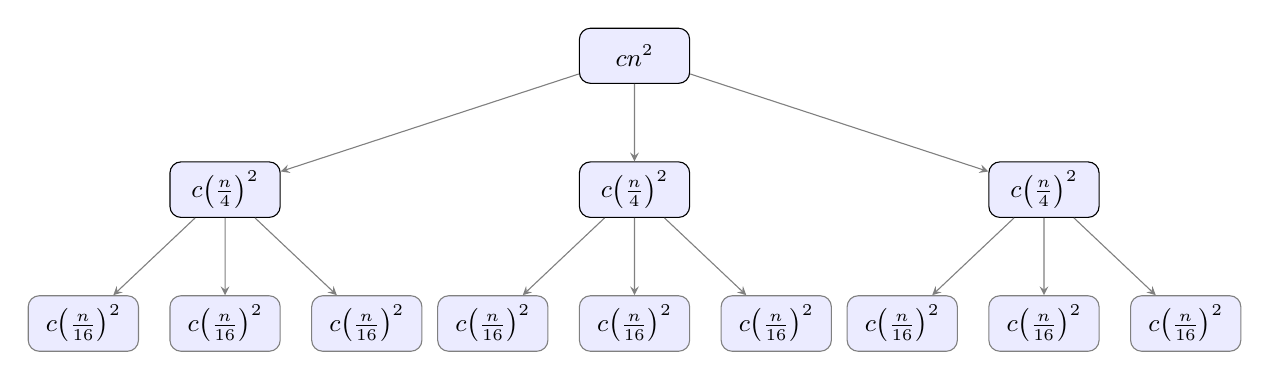
\begin{tikzpicture}[
		level distance=1.7cm,
		level 1/.style={sibling distance=5.2cm},
		level 2/.style={sibling distance=1.8cm},
		every node/.style={draw, rounded corners, fill=blue!8, font=\small, minimum width=1.4cm, minimum height=0.7cm, align=center},
		edge from parent/.style={draw, ->, >=stealth, gray},
		]
		\node {$cn^2$}
		child { node {$c\!\left(\frac{n}{4}\right)^2$}
			child { node {$c\!\left(\frac{n}{16}\right)^2$} }
			child { node {$c\!\left(\frac{n}{16}\right)^2$} }
			child { node {$c\!\left(\frac{n}{16}\right)^2$} }
		}
		child { node {$c\!\left(\frac{n}{4}\right)^2$}
			child { node {$c\!\left(\frac{n}{16}\right)^2$} }
			child { node {$c\!\left(\frac{n}{16}\right)^2$} }
			child { node {$c\!\left(\frac{n}{16}\right)^2$} }
		}
		child { node {$c\!\left(\frac{n}{4}\right)^2$}
			child { node {$c\!\left(\frac{n}{16}\right)^2$} }
			child { node {$c\!\left(\frac{n}{16}\right)^2$} }
			child { node {$c\!\left(\frac{n}{16}\right)^2$} }
		};
	\end{tikzpicture}
	\caption{Albero di ricorsione per $T(n)=3T(\lfloor n/4\rfloor)+\Theta(n^2)$.}
\end{figure}

\subsection{Metodo dell'Esperto}

\begin{softnote}
	Il metodo dell'esperto (o \emph{Master Theorem}) è una \emph{ricetta} diretta: dati i parametri
	$a$, $b$ e la funzione $f(n)$, si confronta $f(n)$ con $n^{\log_b a}$ (il numero di foglie dell'albero)
	e si ottiene la soluzione senza fare conti espliciti sull'albero.
\end{softnote}

\begin{teorema}[Teorema dell'Esperto]
	Date le costanti $a > 0$, $b > 1$ e la funzione $f(n)$ asintoticamente positiva, la ricorrenza
	\[
	T(n) = aT(n/b) + f(n)
	\]
	si risolve come:
	\begin{enumerate}
		\item Se $\exists\,\varepsilon > 0$ t.c.\ $f(n) = O\!\left(n^{\log_b a - \varepsilon}\right)$, allora $T(n) = \Theta(n^{\log_b a})$.
		\item Se $\exists\,k \geq 0$ t.c.\ $f(n) = \Theta\!\left(n^{\log_b a} \lg^k n\right)$, allora $T(n) = \Theta(n^{\log_b a} \lg^{k+1} n)$.
		\item Se $\exists\,\varepsilon > 0$ t.c.\ $f(n) = \Omega\!\left(n^{\log_b a + \varepsilon}\right)$ e $af(n/b) \leq cf(n)$ per qualche $c < 1$ e $n$ sufficientemente grande, allora $T(n) = \Theta(f(n))$.
	\end{enumerate}
\end{teorema}

\begin{hardnote}
	Il teorema \textbf{non si applica} nei casi in cui $f(n)$ non è polinomialmente più grande o più piccola di $n^{\log_b a}$, ad esempio $f(n) = n^{\log_b a} / \log n$: in questo caso nessuno dei tre casi è soddisfatto.
\end{hardnote}

La tabella seguente riassume l'applicazione del teorema ai casi più comuni:

\begin{center}
	\begin{tabular}{llllll}
		\toprule
		\textbf{Ricorrenza} & $a$ & $b$ & $n^{\log_b a}$ & \textbf{Caso} & \textbf{Soluzione} \\
		\midrule
		$T(n) = 9T(n/3) + n$         & 9 & 3 & $n^2$   & 1 & $\Theta(n^2)$          \\
		$T(n) = T(n/2) + \Theta(1)$  & 1 & 2 & $n^0=1$ & 2 ($k=0$) & $\Theta(\log n)$ \\
		$T(n) = 2T(n/2) + n\log n$   & 2 & 2 & $n$     & 2 ($k=1$) & $\Theta(n\log^2 n)$ \\
		$T(n) = 3T(n/4) + n^2$       & 3 & 4 & $n^{\log_4 3} \approx n^{0.79}$ & 3 & $\Theta(n^2)$ \\
		$T(n) = 3T(n/2) + n$         & 3 & 2 & $n^{\log_2 3} \approx n^{1.58}$ & 1 & $\Theta(n^{\log_2 3})$ \\
		\bottomrule
	\end{tabular}
\end{center}

\begin{figure}[H]
	\centering
	\begin{tikzpicture}[
		node distance=1.6cm and 3.8cm,
		box/.style={draw, rounded corners, minimum width=5.2cm, minimum height=1.1cm, align=center, font=\small, fill=gray!10},
		yes/.style={draw, rounded corners, minimum width=4.9cm, minimum height=1.1cm, align=center, font=\small, fill=green!12},
		no/.style={draw, rounded corners, minimum width=4.9cm, minimum height=1.1cm, align=center, font=\small, fill=red!10},
		arrow/.style={->, >=stealth, thick}
		]
		\node[box] (start) {Ricorrenza $T(n)=aT(n/b)+f(n)$\\Calcola $n^{\log_b a}$};
		
		\node[box, below=of start] (c1) {$f(n)=O\!\left(n^{\log_b a-\varepsilon}\right)$?};
		\node[yes, right=of c1] (r1) {Caso 1\\$T(n)=\Theta\!\left(n^{\log_b a}\right)$};
		
		\node[box, below=of c1] (c2) {$f(n)=\Theta\!\left(n^{\log_b a}\lg^k n\right)$?};
		\node[yes, right=of c2] (r2) {Caso 2\\$T(n)=\Theta\!\left(n^{\log_b a}\lg^{k+1}n\right)$};
		
		\node[box, below=of c2] (c3) {$f(n)=\Omega\!\left(n^{\log_b a+\varepsilon}\right)$\\e regolarità?};
		\node[yes, right=of c3] (r3) {Caso 3\\$T(n)=\Theta(f(n))$};
		
		\node[no, below=of c3] (none) {Nessun caso standard\\usa sostituzione o albero};
		
		\draw[arrow] (start) -- (c1);
		\draw[arrow] (c1) -- node[above, font=\scriptsize]{sì} (r1);
		\draw[arrow] (c1) -- node[right, font=\scriptsize]{no} (c2);
		\draw[arrow] (c2) -- node[above, font=\scriptsize]{sì} (r2);
		\draw[arrow] (c2) -- node[right, font=\scriptsize]{no} (c3);
		\draw[arrow] (c3) -- node[above, font=\scriptsize]{sì} (r3);
		\draw[arrow] (c3) -- node[right, font=\scriptsize]{no} (none);
	\end{tikzpicture}
	\caption{Diagramma di flusso per l'applicazione del Teorema dell'Esperto.}
\end{figure}

\begin{nota}
	Un modo intuitivo per ricordare i tre casi: si confronta la \emph{funzione forzante} $f(n)$ con
	il numero di foglie $n^{\log_b a}$.
	\begin{itemize}
		\item \textbf{Caso 1}: le foglie dominano $\Rightarrow$ il costo totale è determinato dalle foglie.
		\item \textbf{Caso 2}: foglie e radice sono bilanciate $\Rightarrow$ ogni livello costa uguale, si moltiplica per $\log n$.
		\item \textbf{Caso 3}: la radice domina $\Rightarrow$ il costo totale è determinato dal livello più alto.
	\end{itemize}
\end{nota}

\subsection{Errori tipici d'esame}
\begin{hardnote}
\textbf{Errore 1:} confondere costo di un livello con costo totale dell'albero di ricorsione.
\end{hardnote}

\begin{hardnote}
\textbf{Errore 2:} nel metodo di sostituzione, concludere erroneamente da
$T(n)\le cn+n=(c+1)n$ che $T(n)=O(n)$.
\end{hardnote}

\begin{hardnote}
\textbf{Errore 3:} applicare il metodo dell'esperto senza verificare la forma $aT(n/b)+f(n)$.
\end{hardnote}

\subsection{Possibili domande d'esame}
\begin{itemize}
	\item Derivare la ricorrenza di MergeSort e risolverla.
	\item Spiegare perché il trucco di Gauss riduce da 4 a 3 moltiplicazioni ricorsive.
	\item Applicare il metodo dell'esperto a $T(n)=2T(n/2)+n\log n$.
	\item Costruire l'albero di ricorsione di $T(n)=3T(n/4)+\Theta(n^2)$.
	\item Motivare i pro/contro della trasformazione ricorsione $\rightarrow$ iterazione.
\end{itemize}
